% !TEX TS-program = LuaLaTex+se

\documentclass[12pt]{report}

\usepackage[autocompile,allowdeprecated=false]{gregoriotex}
\usepackage{ulem}
\usepackage[compact]{titlesec}
\usepackage{graphicx}

\usepackage{romande}
\usepackage[T1]{fontenc}
\input Nouveaud.fd
\newcommand*\initfamily{\usefont{U}{Nouveaud}{xl}{n}}

% choose the language of the document here
\usepackage[latin]{babel}

\usepackage[print,1to1]{booklet}
\pagespersignature{16}
\source{\magstep0}{5.5in}{8.5in}
\target{\magstep0}{11in}{8.5in}
\setpdftargetpages

%%% This function is used at the end of a function which inserts text.  It checks to see if a space should be included at the end of the command, suppressing it if the command is immediately followed by a punctuation character but including it otherwise.
\makeatletter
\newcommand{\punctuationcheck}{%
	\@ifnextchar){\relax}{%
	\@ifnextchar]{\relax}{%
	\@ifnextchar.{\relax}{%
	\@ifnextchar,{\relax}{%
	\@ifnextchar’{\relax}{\ }}}}}%
}
\makeatother

%%%  Code for ordinal numbers.  Note that this code redefines \th to make it produce the superscripted "th" for ordinal numbers and so defines a new command, \thorn, to allow access to the phonetic letter which is usually accessed by that command.
\newcommand{\st}{\textsuperscript{st}\punctuationcheck}
\newcommand{\nd}{\textsuperscript{nd}\punctuationcheck}
\newcommand{\rd}{\textsuperscript{rd}\punctuationcheck}
\let\thorn\th
\renewcommand{\th}{\textsuperscript{th}\punctuationcheck}

%%% Setting up the paper size and margins.
\setlength{\hoffset}{-0.5in}
\setlength{\voffset}{-0.75in}
\setlength{\oddsidemargin}{0in}
\setlength{\evensidemargin}{0in}
\setlength{\topmargin}{0in}
\setlength{\headheight}{0.125in}
\setlength{\headsep}{0.25in}
\setlength{\textheight}{7.0in}
\setlength{\textwidth}{4.5in}
\setlength{\footskip}{0.0in}
\setlength{\marginparwidth}{0.9in}

% formatting titles
\titleformat{\chapter}[block]
	{\centering\Large\bfseries}{}{0pt}{}
\titleformat{\section}[block]
	{\centering\large\bfseries}{}{0pt}{}

% get rid of page numbers
\usepackage{fancyhdr}
\pagestyle{fancy}
\fancyhead{} % clear all header fields
\fancyfoot{} % clear all footer fields
\fancyfoot[C]{\notice}
\renewcommand{\headrulewidth}{0pt}

\def\notice{%
\begin{center}\footnotesize
\ifblackandwhite\else
\tiny Artwork by Fr.~Stephen Reid, OSB, \copyright~1989 St.~Anselm's Abbey\fi
\end{center}
}

% force hyphens between all syllable in a word
\gresethyphen{force}
% tune distances
\grechangedim{afterinitialshift}{2.2mm}{scalable}
\grechangedim{beforeinitialshift}{2.2mm}{scalable}
\grechangedim{annotationraise}{8pt}{scalable}
% format the initial
\grechangestyle{initial}{\initfamily\fontsize{50}{33}\selectfont}
% select the font for the music and tune the glyphs
\gresetgregoriofont[op]{greciliae}
\grechangeglyph{PunctumDescendens}{greciliae}{PunctumDescendens}
% prevents linebreaks mid-word
\xdef\greendofsyllablepenalty{10000}
% red staff lines
\gresetlinecolor{gregoriocolor}

% All antiphons have the same annotation, so we define a convenience function which allows us to manipulate them all at once
\def\commonannotation{%
\greannotation{Ant.}%
\greannotation{\small \textsc{\textbf{ii d}}}%
}

% For getting rid of the images in black and white printing
\newif\ifblackandwhite
\blackandwhitefalse
\ifblackandwhite
	\def\includegraphics[#1]#2{\hbox{}\vfill}
	\colorlet{gregoriocolor}{black}
\fi

\begin{document}

\hbox{}\vfill
\begin{center}
\Huge\bfseries
ANTIPHON\AE\ MAJORES\\
AD MAGNIFICAT.
\vfill
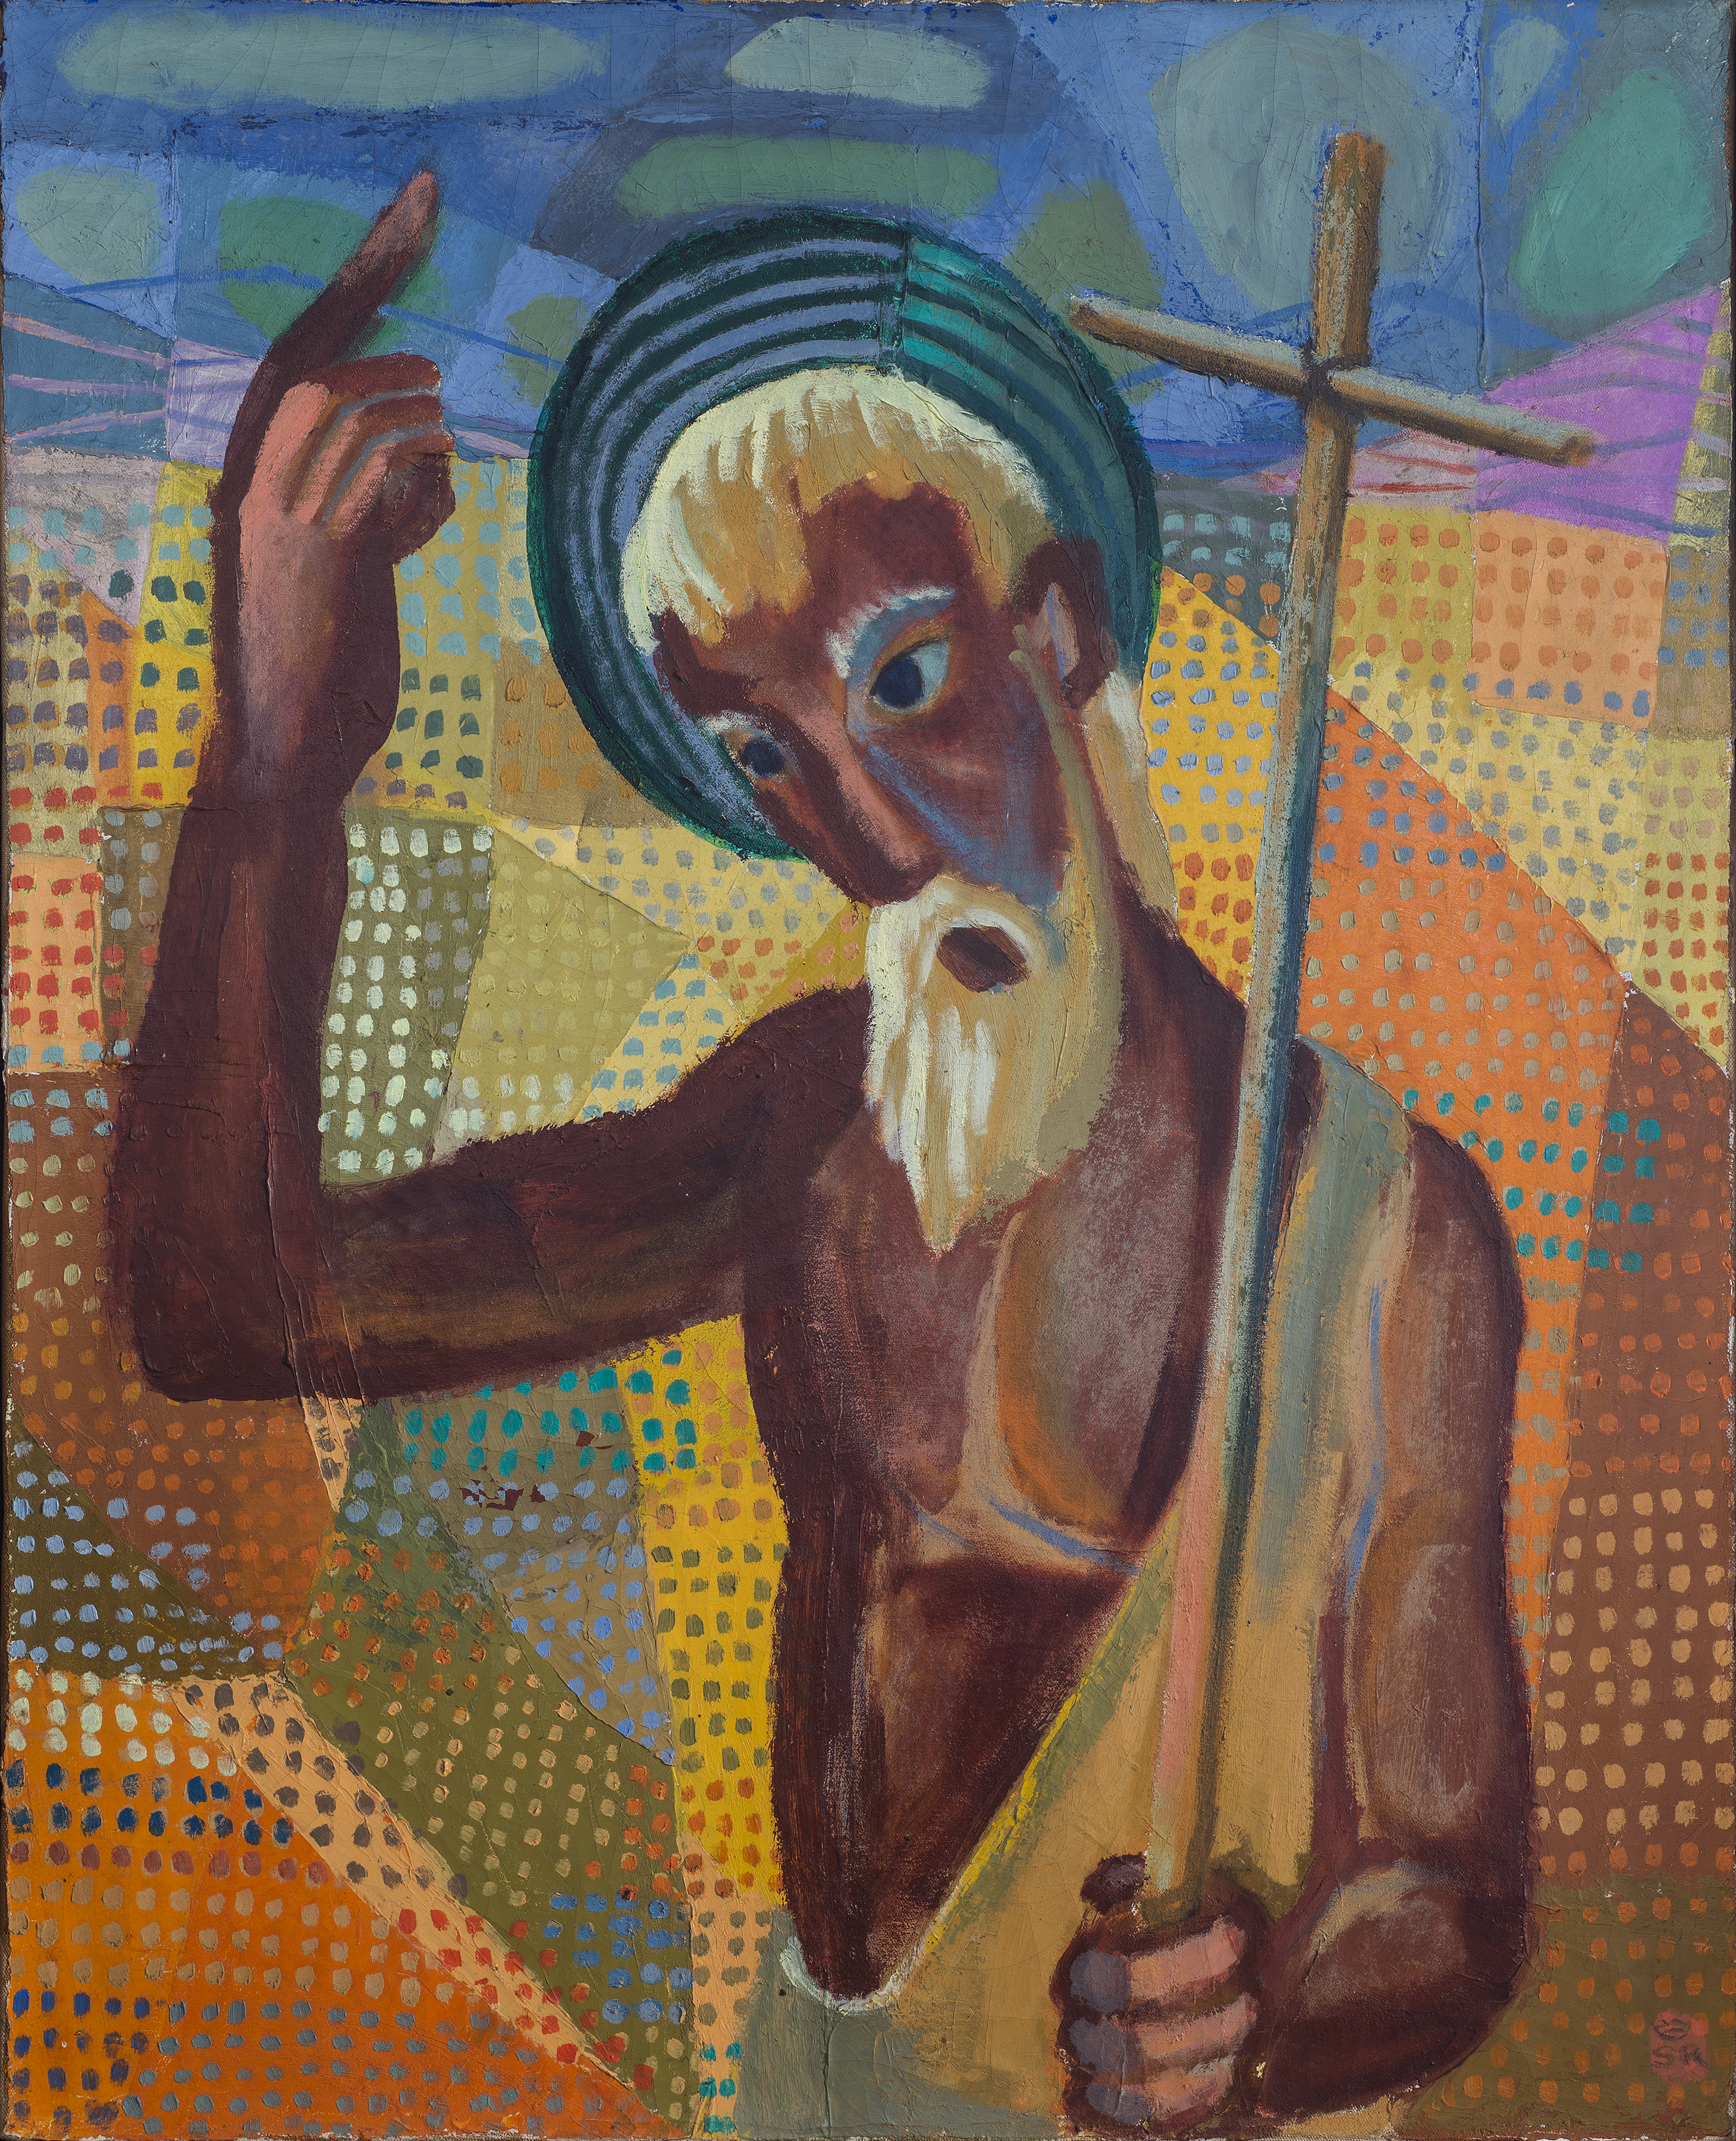
\includegraphics[width=0.5\textwidth]{Images/Saint_John_the_Baptist_(Patterned_Background)}
\vfill
\end{center}
{\small Sequentes Antiphon\ae\ majores ad Magnificat inchoantur die 17 Decembreis, et singul\ae\ ante post Magnificat integr\ae\ sicut Duplicius dicuntur per ordinem usque ad diem ante Vigiliam Nativitatis.  Se vero Festum fuerit, dicuntur post Orationem Festi, pro commemoratione Adventus.
\vfill
}

\pagebreak
\begin{center}\includegraphics[height=0.3\textheight]{Images/Sapientia}\end{center}
\section*{O Wisdom (December 17\th)}
\commonannotation
\gregorioscore{Scores/O_Sapientia}
\vfill

\pagebreak
\begin{center}\includegraphics[height=0.3\textheight]{Images/Adonai}\end{center}
\section*{O Lord (December 18\th)}
\commonannotation
\gregorioscore{Scores/O_Adonai}
\vfill

\pagebreak
\hbox{}\vfill
\section*{O Root of Jesse (December 19\th)}
\commonannotation
\gregorioscore{Scores/O_radix_Jesse}
\vfill

\pagebreak
\begin{center}\includegraphics[height=0.35\textheight]{Images/clavis}\end{center}
\section*{O Key of David (December 20\th)}
\commonannotation
\gregorioscore{Scores/O_clavis_David}
\vfill

\pagebreak
\hbox{}\vfill
\section*{O Rising Sun (December 21\st)}
\commonannotation
\gregorioscore{Scores/O_Oriens}
\vfill

\pagebreak
\hbox{}\vfill
\section*{O King of Nations (December 22\nd)}
\commonannotation
\gregorioscore{Scores/O_Rex_gentium}
\vfill

\pagebreak
\hbox{}\vfill
\section*{O Emmanuel (December 23\rd)}
\commonannotation
\gregorioscore{Scores/O_Emmanuel}
\vfill

\end{document}
